% Implementation: Iterative over stack 
% Spec: Recursive operation over an inductive data type for trees
\begin{frame}{TreeHash}

\begin{columns}[c,onlytextwidth]
\begin{column}{0.40\textwidth}
\begin{itemize}
  \setlength{\itemsep}{4mm}
  \item Computes the root of a Merkle subtree from its leaves.
  \item \textbf{Security Specification}: Expressed as a recursive function over an inductive data type for trees.
  \item \textbf{RFC Specification}: Iterative function that makes use of a stack for storing intermediate nodes.
\end{itemize}
\end{column}
\begin{column}{0.57\textwidth}
  \centering
  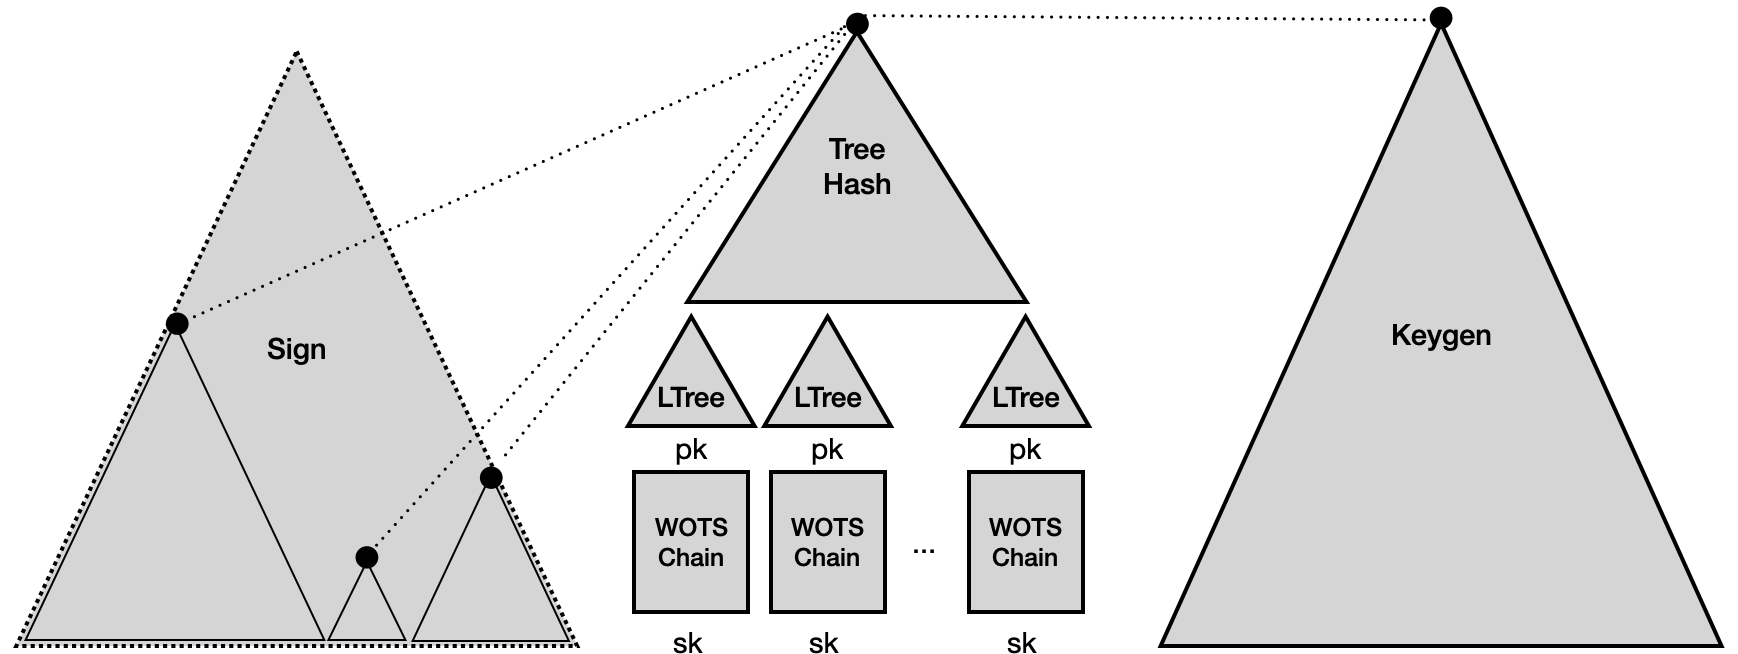
\includegraphics[width=\linewidth]{img/treehash.png}
\end{column}
\end{columns}
\end{frame}
